\documentclass{beamer}

%\usepackage{beamerthemesplit} // Activate for custom appearance
%\usepackage\{beamercolorthemedove}
%\setbeamertemplate{footline}[textline]{
%\includegraphics[width=\paperwidth]{figures/datacron_logo.png}}
%}

\usepackage{textpos}
\usepackage{graphicx}
\usepackage{datetime}
\usepackage{tikz}
\usepackage[export]{adjustbox}
 \usepackage{natbib}
 
 \usepackage{pgf}
 \usepackage{tikz}
 \usetikzlibrary{arrows,automata}
 %json%
\usepackage{minted}
%sudo apt-get install python-pygments
\usecolortheme{dove}

\def\datacronlogo{%
  \resizebox{!}{2.5ex}{\includegraphics{figures/datacron_logo.png}%
}
}
\def\eclogo{
  \resizebox{!}{2.5ex}{\includegraphics{figures/ec_logo.png}%
}
}
\def\horizonlogo{%
  \resizebox{!}{2.5ex}{\includegraphics{figures/horizon_logo.png}%
}
}


\def\fraunhoferlogo{%
	\resizebox{!}{2.5ex}{\includegraphics{figures/iais.pdf}%
	}
}
\def\unibonnlogo{%
	\resizebox{!}{2.5ex}{\includegraphics{figures/logo.pdf}%
	}
}
%\includegraphics[width=\paperwidth]{figures/datacron_logo.png}}

\title{	Distributed Online Learning for Large-scale Pattern Prediction over Real-time Event Streams}
%\author[shortname]{Author Name 1 \inst{1} \and Author Name 2 \inst{2}}
%\institute[shortinst]{\inst{1} affiliation for author1 \and %
 %                     \inst{2} affiliation for author2}
%\date{\today}

\defbeamertemplate*{footline}{example theme}
{%
    \begin{beamercolorbox}[wd=\paperwidth,ht=2.5ex,dp=1.125ex,%
        leftskip=.3cm,rightskip=.3cm plus1fil]{separation line}
        \usebeamerfont{section in head/foot}%
        \unibonnlogo\hfill\insertshorttitle\hfill\dmyydate \today\hfill \thepage \hfill \fraunhoferlogo
            \end{beamercolorbox}
}
\begin{document}


\frame
{
	\frametitle{Event Forecasting with Pattern Markov
		Chains  }
	\framesubtitle{ How does it work?}
	\begin{itemize}
		\item<only@1> The pattern \boldmath$P=b\cdot c$ is converted to $DFA$ with $\Sigma=\{a,b,c\}$. 
		 \begin{figure}[ht]
	\begin{center}
		
		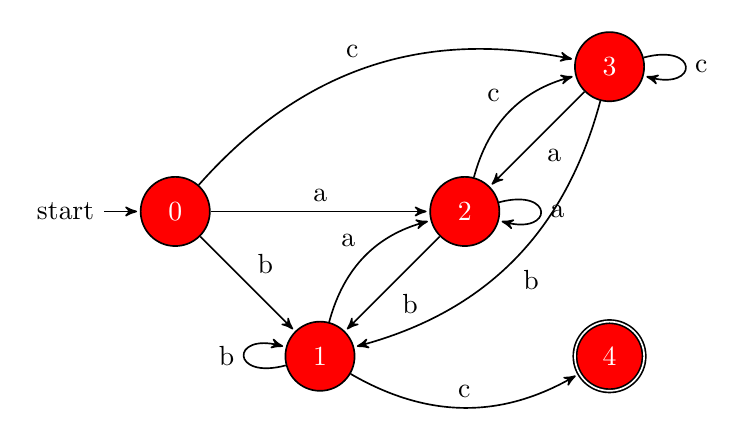
\begin{tikzpicture}[->,>=stealth',shorten >=1pt,auto,node distance=2.6cm,
		semithick]
		\tikzstyle{every state}=[fill=red,text=white]		 
%\begin{tikzpicture}[node distance=7em, scale=1, transform shape]
\node[state, initial] (s0) {$0$};
\node[state, below right of=s0] (b) {$1$};

\node[state, above right of=b] (a) {$2$};
\node[state, above right of=a] (c1) {$3$};
\node[state,accepting,below right of=a] (cF) {$4$};
\path (s0) edge              node {b} (b)
	       edge              node {a} (a)
	       edge   [bend left]  node {c} (c1)
	       
	       (a) edge              node {b} (b)
	                edge     [loop right]         node {a} (a)
	                edge   [bend left]  node {c} (c1)
	                
	        (b) edge   [loop left]           node {b} (b)
	        edge   [bend left]           node {a} (a)
	        edge  [bend right]   node {c} (cF)
	        
	        (c1) edge     [ bend left]        node {b} (b)
	        edge              node {a} (a)
	        edge   [loop right]  node {c} (c1)
	        
	        ;

\end{tikzpicture}
\end{center}
\caption[]{$ Q=\{0,1,2,3,4\}$       $m=1$}
\end{figure}
		
	\end{itemize}
}



\frame
{
	\frametitle{Event Forecasting with Pattern Markov
		Chains}
	\framesubtitle{How does it work?}
	\begin{itemize}
		\item<only@1> \begin{equation*}
		\label{eq:matrix_example}
		\boldsymbol{\hat{M}\ for\ mc} = 
		\begin{Bmatrix} 
		a \\ b \\ c \\
		\end{Bmatrix}
		\begin{pmatrix} 
		p_{a,a}	    &. 	&  	p_{a,c} \\
		.	        &. 	&  	.       \\
		p_{c,a}	    &. 	&  	p_{c,c} \\
		\end{pmatrix}
		\end{equation*}
		
		\item<only@1> 
		\begin{equation*}
		\label{eq:matrix_example}
		\boldsymbol{M\ for\ pmc} = 
		\begin{Bmatrix} 
		0 \\ 1 \\ 2 \\ 3 \\4
		\end{Bmatrix}
		\begin{pmatrix} 
		p_{0,0}	    &. 		&. 		& . &  	p_{0,4} \\
		. 		    & .		& .	& .	& . \\
		.		    & .		& .		& .	& . \\
		.			& .		& .		& .	& .\\
		0			& .			& .		& .	&p_{4,4}
		\end{pmatrix}
		\end{equation*}
		
		\item<only@1> can we find $p_{i,j}$  based on $\boldsymbol{\hat{M}}$ ? 
		\begin{equation}
		\label{eq:pi_estim}
		p_{i,j}=\sum_{} p_{x,y}
		\end{equation}.
		such that $x \in incoming\ edges\ to\ i$ 	and  $y \in outgoing\ edges\ from\ j\ to\ i$
		
	\end{itemize}
}



\end{document}
